% \documentclass[10pt,conference,compsoc]{IEEEtran}
% \documentclass[10pt,journal,compsoc]{IEEEtran}
\documentclass[a4paper]{article}



\usepackage[T1]{fontenc}
\usepackage[utf8]{inputenc}
\usepackage{authblk}
\usepackage{hyperref}
\usepackage{cite}
\usepackage{graphicx}
\usepackage{float}
\usepackage{textcomp}
% \usepackage{wrapfig}

\renewcommand\thesection{\arabic{section}}
\renewcommand\thesubsection{\thesection.\arabic{subsection}}

\makeatletter
\def\@seccntformat#1{\@ifundefined{#1@cntformat}%
   {\csname the#1\endcsname\space}%    default
   {\csname #1@cntformat\endcsname}}%  enable individual control
\newcommand\section@cntformat{\thesection.\space}       % section-level
\newcommand\subsection@cntformat{\thesubsection \space} % subsection-level
\makeatother

\hypersetup{
    colorlinks,
    citecolor=black,
    filecolor=black,
    linkcolor=black,
    urlcolor=black
}

\def\IEEEcompsocdiamondline{}

\renewcommand{\abstractname}{\large ABSTRACT\\}
\makeatletter
  \ifCLASSOPTIONconference% compsoc conference
\def\abstract{\normalfont\@IEEEtweakunitybaselinestretch{1.19}\bfseries
% \def\abstract{\itshape\@IEEEtweakunitybaselinestretch{1.15}\bfseries
    \if@twocolumn
      \@IEEEabskeysecsize\noindent\textbf{\abstractname}\relax
    \else
      \bgroup\par\addvspace{0.5\baselineskip}\centering\vspace{-1.78ex}\@IEEEabskeysecsize\textbf{\abstractname}\par\addvspace{0.5\baselineskip}\egroup\quotation\@IEEEabskeysecsize%
    \fi\@IEEEgobbleleadPARNLSP}
\makeatother

\renewcommand{\abstractname}{\large ABSTRACT\\}
\let\oldabstract\abstract
\renewcommand\abstract{%
  \begingroup
  \let\textbf\relax
  \oldabstract
  \endgroup
  \bfseries
}        

\title{\LARGE \bf 
A Distributional Semantics Model for Metaphor Detection
}

\renewcommand\Authfont{\fontsize{13}{14.4}\selectfont}
\renewcommand\Affilfont{\fontsize{10}{10.8}\selectfont}

\author{ Jasim Ahmed , Mirza Mustansar Baig}
\affil { Department of Computer Science,  Universität Passau }

\begin{document}
\maketitle

\section{ABSTRACT}
Metaphors are an integral part of any language. They bring life to the effective communication. Many approaches have been proposed to detect the sense of a phrase being used as literal or metaphorical. Metaphors are generally compositional and this composition can be translated to a source domain of a concept to a target domain of a different but related concept. Compositional distributed semantic models provide a good way to understand this composition and help in identifying the sense of a phrase to be used as literal or metaphorical. It is also important to know the context of a phrase which can help in figuring out the sense and this context can be analyzed using vectors. Using Distributional Semantic Models, phrases can be identified as being used  metaphoric by applying algebraic expressions on vectors.

\section{INTRODUCTION}
Metaphors are an interesting way of communication. It is generally a comparison referring to a person, place or thing as being something else i.e “Your brain is a computer”. In this example, brain is referred to as computer due to its capability to solve complex problems in less time. One of the literal ways of conveying this idea would be “You are a smart person with extreme mental capabilities”. Metaphors can be divided into two categories, conceptual metaphors and linguistic metaphors. Linguistic metaphors are instantiations on the broader category of conceptual metaphors. While instantiating the linguistic metaphor, there is always a mapping that is performed from the source of the concept to the target of that concept. In the metaphor, “Your brain is a computer”, the source domain of “Human Intellect” is mapped on the target domain of “Digital Computation”. According to the Conceptual Metaphor Theory, this mapping is always done systematically and hence can be calculated in the sentences to figure out the sense being literal or metaphorical. Metaphorical sense is not the characteristic of an individual word, instead it is composed by the mapping of one domain to another domain. \\

The metaphorical senses of sentences have been detected by many techniques including Distributional Statistics(DS), Vector Space Models(VSM), Distributional Semantic Models(DSM), Compositional Distributional Semantic Models(CDSM) etc. An interesting characteristic of metaphors is that their metaphorical or literal sense can be detected by the way they are composed using source and target domain e.g “heavy processing”, “heavy logic” are composed by inter-play of source and target domains.\\

This compositionality can be determined by the compositional distributional semantic models (CDSM) in which phrases are treated as vectors. From these phrases, nouns are represented as vectors and adjectives as matrices. Due to the systematic composition of the phrases, the context of the phrases can also be computed using CDSM.\\

We are using the idea of adjective-noun phrase vectors. Once the vectors are created, these vectors are fed to the classifier as attributes. Based on these attributes, classifier, classifies the phrase and annotates the phrase as being used in literal or metaphorical sense.

\begin{figure}[h!]
  \centering
  
\includegraphics[width=0.7\textwidth]{Time-is-Money}
  \caption{An example of Metaphor}
\end{figure}

\section{Similar Ideas}
Two similar ideas exist along with the metaphors in phrase compositions. These are as follows:

\subsection{Similie}
It refers to a comparison that is done using the word “as” e.g “as bright as a star”.

\subsection{Idioms}
It refers to an expression that means something else than the words say.

\subsection{Morphism}
The structure of the metaphors can also be understood by the idea of “morphism” which is a concept given by “Category Theory”. Morphism is the transformation of an object to another object in such a way that it preserves some of the structure of original object. This transformation of objects can be explored to understand the composition of the metaphor.

\subsection{Polysemy}
A polyseme is a word or phrase with different, but related senses. This property of the word introduces ambiguity while understanding it and can be done if the context of the word is given. CDSMs can avoid this ambiguity while making sense of a word since it contains matrices for adjectives which already contain the context of the word.

\section{Background}

\subsection{Distribution Theory}
The distributional hypothesis in linguistics is that words that occur in similar contexts tend to have similar meanings (Harris, 1954). This hypothesis is the justification for  applying the DSM to measuring word similarity. A word may be represented by a vector in which the elements are derived from the occurrences of the word in various contexts. If words have similar row vectors in a word context matrix, then they tend to have similar meanings.

\subsection{Compositional Distributed Semantic Model}
The main idea behind the CDSMs is to perform algebraic expressions on the vector representation of words and phrases and from those expressions, learn the composition of phrases. With this knowledge about the composition, we can detect whether the phrase is used in literal or metaphorical sense.

\subsection{Krishnakumaran and Zhu Metaphor Detection}
They focused on detecting whether an adjective-noun phrase is used in a literal or metaphorical way. They kept the count of adjective-noun co-occurrence in the dataset and the WordNet hyponym and hypernym relations. The main idea is that if some certain noun and hypernym/hyponym do not occur very frequently with some certain adjective then this phrase is used as a metaphor.

\section{Main Approach}
Our main approach is inspired by all the ideas above. Following is the main activity/flow diagram which describes the overall structure of the approach taken.

\begin{figure}[h!]
  \centering
  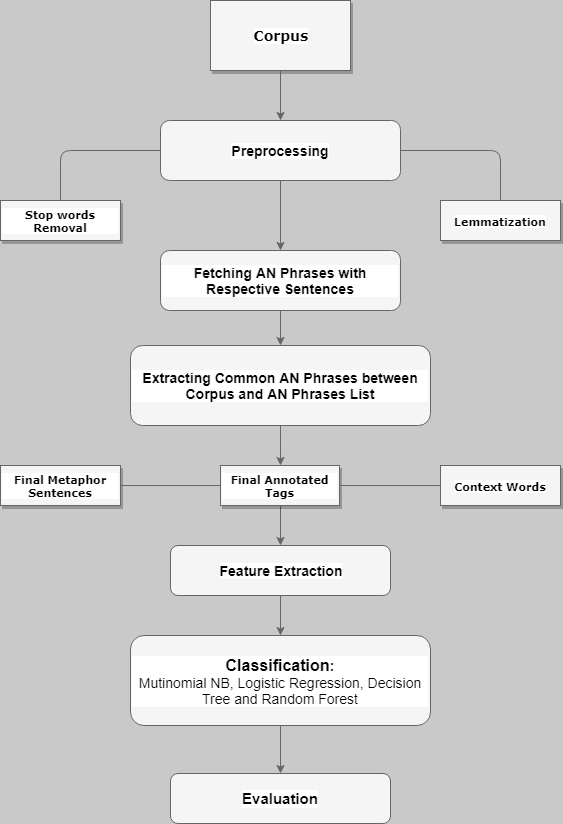
\includegraphics[width=0.9\textwidth]{FlowChart}
  \caption{Flow Diagram}
\end{figure}

\subsection{Corpus}
We chose Brown corpus from NLTK. It contains different kinds of categories including Adventure, Editorial, Fiction, Government, Hobbies, Humor, Learned, Lore, Mystery, News, Religion, Reviews, Romance and Science Fiction. Many of these categories contain phrases that are used in metaphorical senses. 

\subsection{Pre-processing}
Brown corpus is already POS tagged so we did not have to POS tag it on our own. POS tagging helps in finding the Noun and Adjectives which will be used in order to annotate the phrases later on. For simplicity, we are working with the universal tag set which simplifies and limits the tags to their very basic form.\\
In order to save processing time, stop words are removed from the corpus sentences at the first step. After that these sentences are lemmatized to save the processing time even further. In the next step, all the adjective noun(AN) phrases are extracted from the sentences. This is created into a tuple having the sentence as the first element and the AN-phrase as the second element of the tuple. the reason we are extracting the AN-phrase from the sentences is that we will use these phrases later on to extract all the matching phrase sentence from the corpus.\\
Now that we have all the phrases and their respective sentences, we can compare these phrases with the AN-phrase set and only take the matching phrase sentences. The rest of the sentences are discarded. This step significantly reduces the our matrix computation later on because the number of sentences are reduced to only the desired AN-phrase matching set. While calculating the common sentences between the corpus sentences and the AN-phrase set, sentences are annotated and context words are fetched at the same time. 
Since the Brown corpus is very large and requires a significant amount of processing time in order to look at all the phrases and decide whether it is used as literal or metaphor, we fetched all the common words and phrases from the corpus. These phrases are then fed to term-document matrix afterwards for generating the vectors for the phrases.

\subsection{AN-Phrase Dataset}
We are using a data set of adjective-noun phrases. Each phrase in the data set was annotated manually by a group of people  as being used either literally or metaphorically. This data set was created by E. Dario Gutierrez, Ekaterina Shutova, Tyler Marghetis and Benjamin K. Bergen. The data set was created by choosing 23 adjectives that can possibly have both literal as well as metaphorical senses. Each of these adjectives behave as source-domain words while constructing conceptual metaphors described by Conceptual Metaphor Theory. The annotated data set is publicly available at http:
//bit.ly/1TQ5czN

\subsection{Sentence Annotation(Metaphor/Literal)}
The common extracted sentences need to be annotated as literal or metaphorical. This annotation is the key to classification. A sentence is annotated based on the annotation of the respective AN-Phrase. If the AN-Phrase has metaphorical sense annotation then the sentence is annotated as "Y" otherwise it gets annotated as "N".

\subsection{Context Words}
The context words are the words that are obtained by removing the AN-Phrase from the actual corpus sentence. The remaining words are the words that are used as the context of that particular AN-Phrase. This approach will help us making the co-occurrence matrix with exact context of a AN-Phrase.  

\subsection{Feature Extraction}
Based on the above mentioned AN-phrase data set, we extracted all the sentences from the data set that involve these phrases. With this step, we reduced the processing time of creating the vectors for the phrases from the Brown corpus. Without this, we had to check all of the sentences and construct the matrices afterwards. Now we can only work with these selected sentences and find out about their usage sense.
After finding all the relevant phrases along with their annotation tags and context words from the corpus, a document-term matrix was constructed. In this matrix, the documents are the sentences that are extracted based on the AN phrase set and the terms are the common words in the whole corpus. The resulting matrix is the collection of frequency vectors. Each vector represents a sentence(document) which is either used in literal or metaphorical form. This vector inherently contains all of the context of the phrase that needs to be looked at for its sense understanding.

\subsection{Classification}
The classification technique is a systematic approach to build classification models from an input data set. For example, decision tree classifiers, rule-based classifiers, neural networks, support vector machines, and naive Bayes classifiers are different technique to solve a classification problem. Each technique adopts a learning algorithm to identify a model that best fits the relationship between the attribute set and class label of the input data. Therefore, a key objective of the learning algorithm is to build predictive model that accurately predicts the class labels of previously unknown records. Since the data we are working on is multi-label data, one of the obvious choices for the classifier is Multinomial Naive Bayes classifier. 

\subsubsection{Naive Bayes}
The Naive Bayes Classifier technique is based on the so-called Bayesian theorem and is particularly suited when the dimensionality of the inputs is high. Despite its simplicity, Naive Bayes can often outperform more sophisticated classification methods.

\begin{figure}[h!]
  \centering
  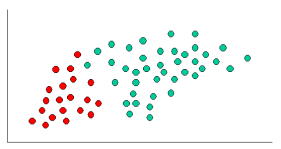
\includegraphics[width=0.7\textwidth]{NaiveBayes}
  \caption{Naive Bayes}
\end{figure}

To demonstrate the concept of Naïve Bayes Classification, consider the example displayed in the illustration above. As indicated, the objects can be classified as either GREEN or RED. Our task is to classify new cases as they arrive, i.e., decide to which class label they belong, based on the currently exiting objects.
\\
Since there are twice as many GREEN objects as RED, it is reasonable to believe that a new case (which hasn't been observed yet) is twice as likely to have membership GREEN rather than RED. In the Bayesian analysis, this belief is known as the prior probability. Prior probabilities are based on previous experience, in this case the percentage of GREEN and RED objects, and often used to predict outcomes before they actually happen.
\\
Since Naive Bayes uses clustering technique, this technique is useful for metaphor classification. As the vectors are given as the X component and annotation tags are given as the Y component, Naive Bayes clusters the literal vectors in in one cluster and metaphor classifier in another cluster, hence classifies the sentences.


\subsubsection{Decision Tree}
The decision tree classifiers organized a series of test questions and conditions in a tree structure. The following decision tree is for predicting whether the person cheats. In the decision tree, the root and internal nodes contain attribute test conditions to separate records that have different characteristics. All the terminal nodes are assigned a class label either Yes or No.
\begin{figure}[h!]
  \centering
  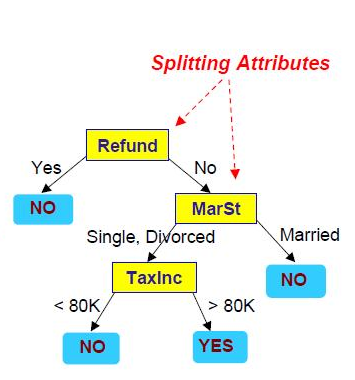
\includegraphics[width=0.5\textwidth]{DecisionTree}
  \caption{Decision Tree}
\end{figure}

Once the decision tree has been constructed, classifying a test record is straightforward. Starting from the root node, we apply the test condition to the record and follow the appropriate branch based on the outcome of the test. It then leads us either to another internal node, for which a new test condition is applied, or to a leaf node. When we reach the leaf node, the class label associated with the leaf node is then assigned to the record. As shown in the following figure it traces the path in the decision tree to predict the class label of the test record, and the path terminates at a leaf node labeled NO.
\\
We chose the decision tree classifier because its works on the binary decision of to be or not to be. We need the classifier to classify whether a certain phrase is used in literal or metaphorical sense.

\subsection{Random Forest}
Random Forests are an ensemble of k untrained Decision Trees (trees with only a root node) with M bootstrap samples (k and M do not have to be the same) trained using a variant of the random subspace method or feature bagging method. The procedure for training a random forest is as follows:

\begin{enumerate}
    \item At the current node, randomly select p features from available features D. The number of features p is usually much smaller than the total number of features D.
    \item Compute the best split point for tree k using the specified splitting metric (Gini Impurity, Information Gain, etc.) and split the current node into daughter nodes and reduce the number of features D from this node on.
    \item Repeat steps 1 to 2 until either a maximum tree depth l has been reached or the splitting metric reaches some extrema.
    \item Repeat steps 1 to 3 for each tree k in the forest. Vote or aggregate on the output of each tree in the forest.
\end{enumerate}
\\
Random Forest is a special case of Decision Tree and can be used for the metaphor detection as explained earlier.  



\section{Case Study}
Let’s take an example to better understand how the approach works with a case study. Let for example consider the following sentences as the Corpus which needs to be classified.
\begin{itemize}
    \item S1 = “Simon is a straight-A student.”
    \item S2 = “Simon is a bright boy.”
    \item S3 = “Simon’s shoes have bright colors.”
    \item S4 = “Simon lives near Passau.”
\end{itemize}
S1, S2, S3 and S4 represent documents in a corpus. Let us also consider the following AN phrase set:

\begin{itemize}
    \item P1 = “bright boy”
    \item P2 = “bright color”
\end{itemize}

Where P1 and P2 represent the phrases from an already created AN-Phrase (Adjective Noun Phrase) set. The AN-Phrase set contains phrases along with their senses being either metaphorical or literal. In the first step of preprocessing, we take all the sentences and remove all the stop words from them. After the stop words removal and lemmatization the sentences look as follows:

\begin{itemize}
    \item S1 = “Simon straight-A student.”
    \item S2 = “Simon bright boy.”
    \item S3 = “Simon shoe bright color.”
    \item S4 = “Simon live near Passau.”
\end{itemize}

 In the next step, only the sentences that involve P1 and P2 are kept for further processing and the remaining data will be discarded. In our case study, since only S2 and S3 match with P1 and P2, so we keep these and discard S1 and S4.
\\
Now we need to annotate S2 and S3 and this annotation will be used for the classification step. These sentences are annotated according to the annotation of P1 and P2 which was given in the AN-Phrase data set. After the preprocessing of the raw data, we are all set to create a word-context(document-term) co-occurrence matrix. This matrix is created using tf-idf technique which will put the S2 and S3 on the left hand side and all the context words within these sentences on top of the matrix. The matrix looks like the following:

\begin{figure}[h!]
  \centering
  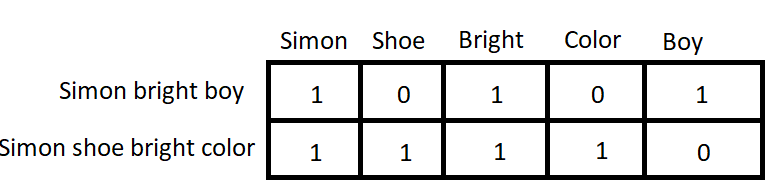
\includegraphics[width=0.7\textwidth]{Tf_Idf}
  \caption{TF-IDF Matrix}
\end{figure}

This matrix is then fed into the classifier which then learns the vectors based on the annotation tags and classifies the test vectors as being literal or metaphorical. In our case study, the classifier learns that the metaphorical vectors will look like the following:

\begin{figure}[h!]
  \centering
  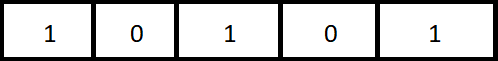
\includegraphics[width=0.7\textwidth]{Tf_Idf_Y}
  \caption{TF-IDF Metaphorical Vector}
\end{figure}

And the literal vectors will look as below:

\begin{figure}[h!]
  \centering
  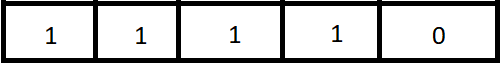
\includegraphics[width=0.7\textwidth]{Tf_Idf_N}
  \caption{TF-IDF Literal Vector}
\end{figure}

Of course in real time classification, the data is always huge and classifier needs time before it learns all the patterns of both literal and metaphorical senses from the train data.

\section{Evaluation and Results}
In this section we have shown all the results after applying different kinds of classifiers. These results have been displayed on Bar Charts showing the comparative accuracy, precision, recall and F1 scores.

\subsection{Train Test Split}
The Data in "Word Context Matrix" is split into training data and test data using "Train Test Split". The mean accuracy for Multinomial Naive Bayes Classifier and Decision Tree is shown in the following Figure.\ref{fig:train test split}
\begin{figure}[H]
 \centering
   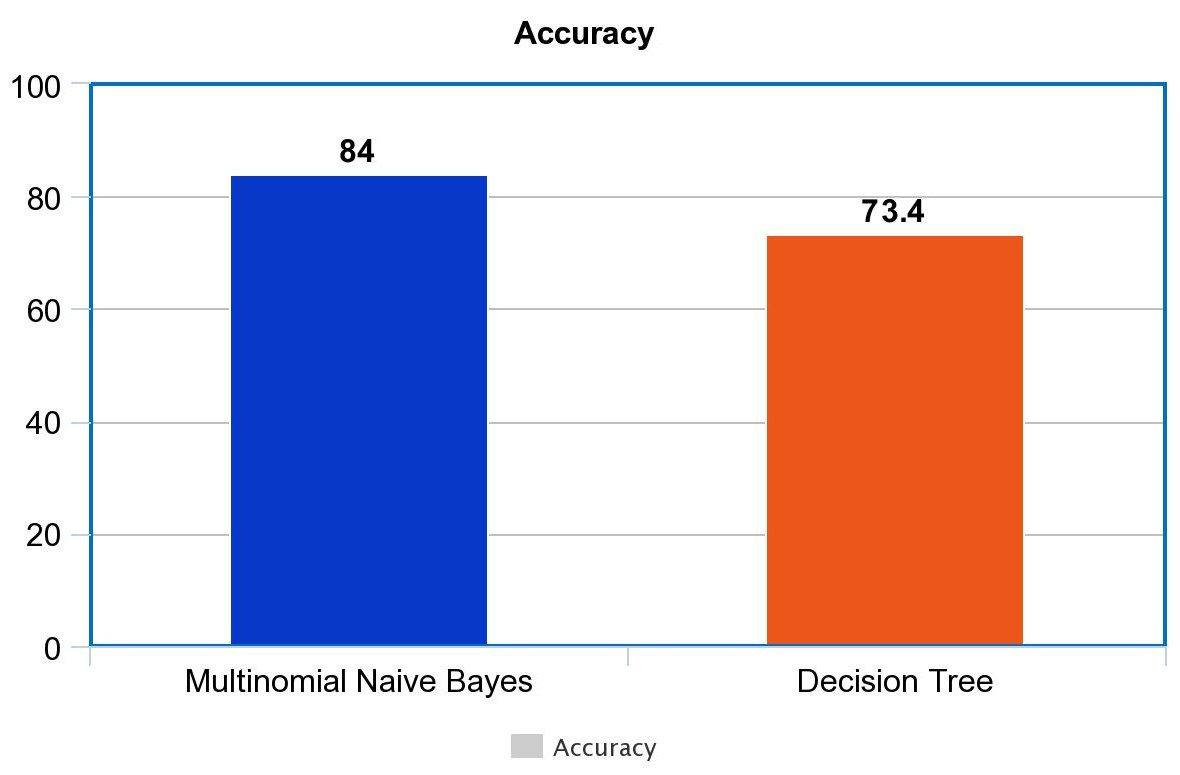
\includegraphics[width= 8cm]{traintestsplit}
\caption{Classifiers}
  \label{fig:train test split}
\end{figure}
\\
\subsection{Repeated K-Fold}
The Data in "Word Context Matrix" gets split into k subsets, and trained on one of the k-1 subset and the last subset is held for test. Repeated K-Fold is used in estimating whether our model is over-fitting or under-fitting.
\\
Applying repeated K-Fold on four different classifiers, the mean accuracy varies a lot on given test data and labels. As shown in Figure \ref{fig:Repeated KFold Accuracies}
\begin{figure}[H]
 \centering
   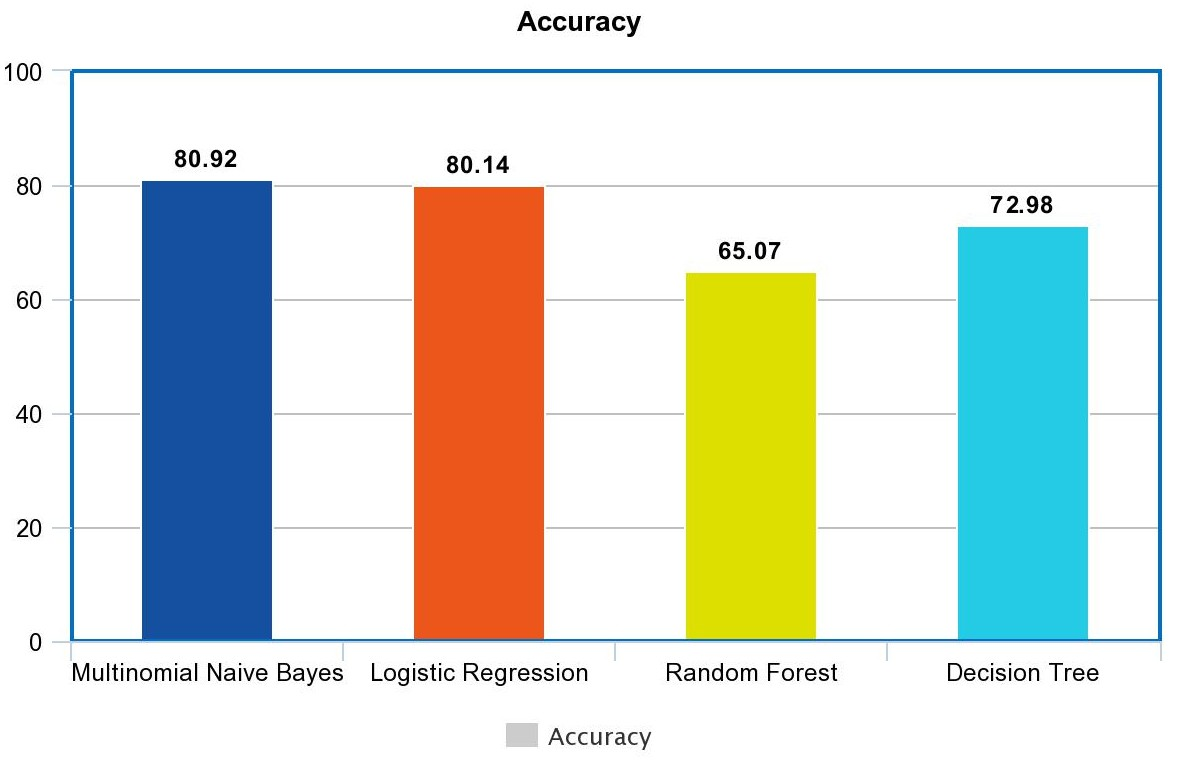
\includegraphics[width= 8cm]{RepeatedKFoldAccuracies}
\caption{Accuracy}
  \label{fig:Repeated KFold Accuracies}
\end{figure}

The comparative mean precision is shown in the following Figure \ref{fig:Repeated KFold Precision}
\begin{figure}[H]
 \centering
   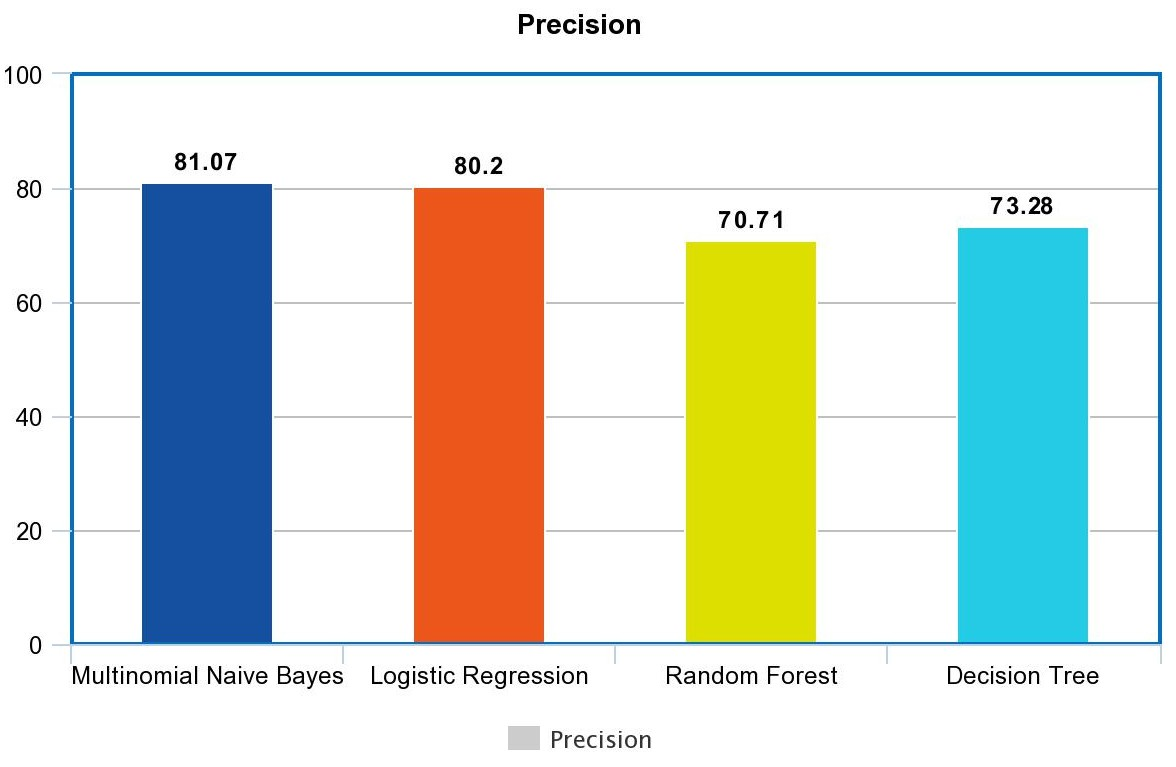
\includegraphics[width= 8cm]{RepeatedKFoldPrecision}
\caption{Precision}
  \label{fig:Repeated KFold Precision}
\end{figure}

The mean Recall is shown in the following Figure \ref{fig:Repeated KFold Recall}
\begin{figure}[H]
 \centering
   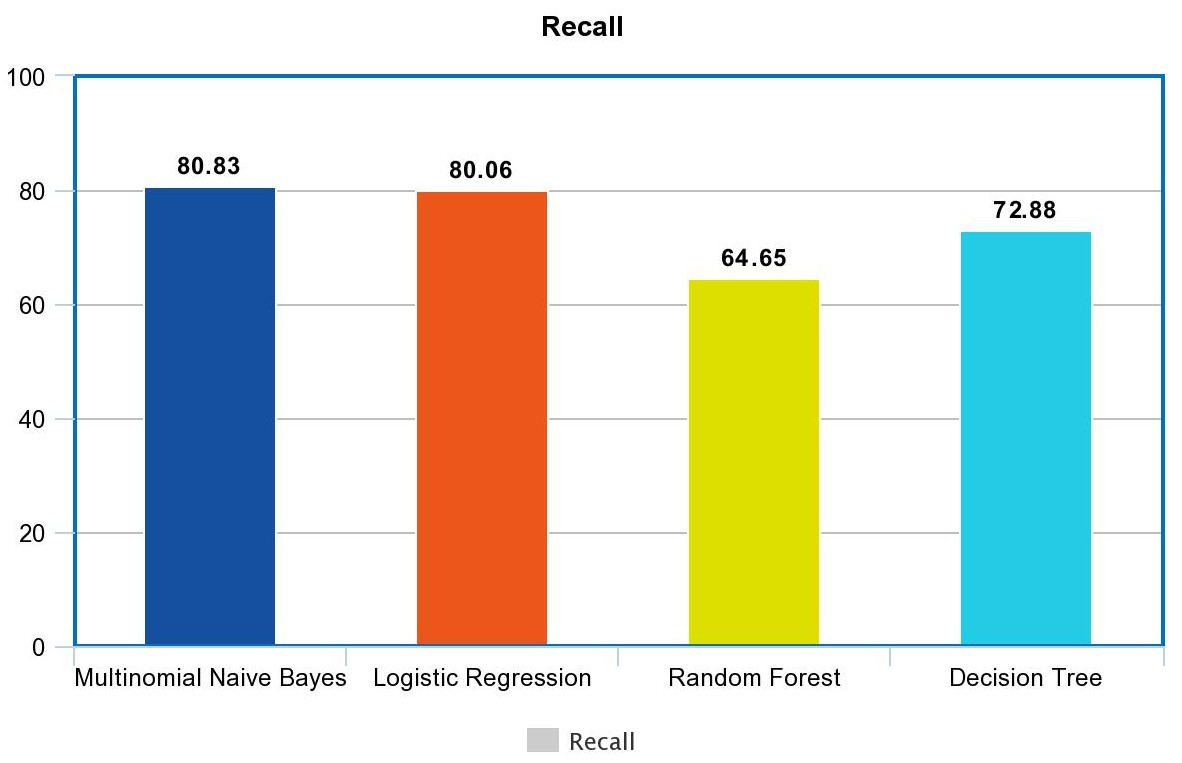
\includegraphics[width= 8cm]{RepeatedKFoldRecall}
\caption{Recall}
  \label{fig:Repeated KFold Recall}
\end{figure}

The mean F1\_score is shown as in Figure \ref{fig:Repeated KFold F1_score}
\begin{figure}[H]
 \centering
   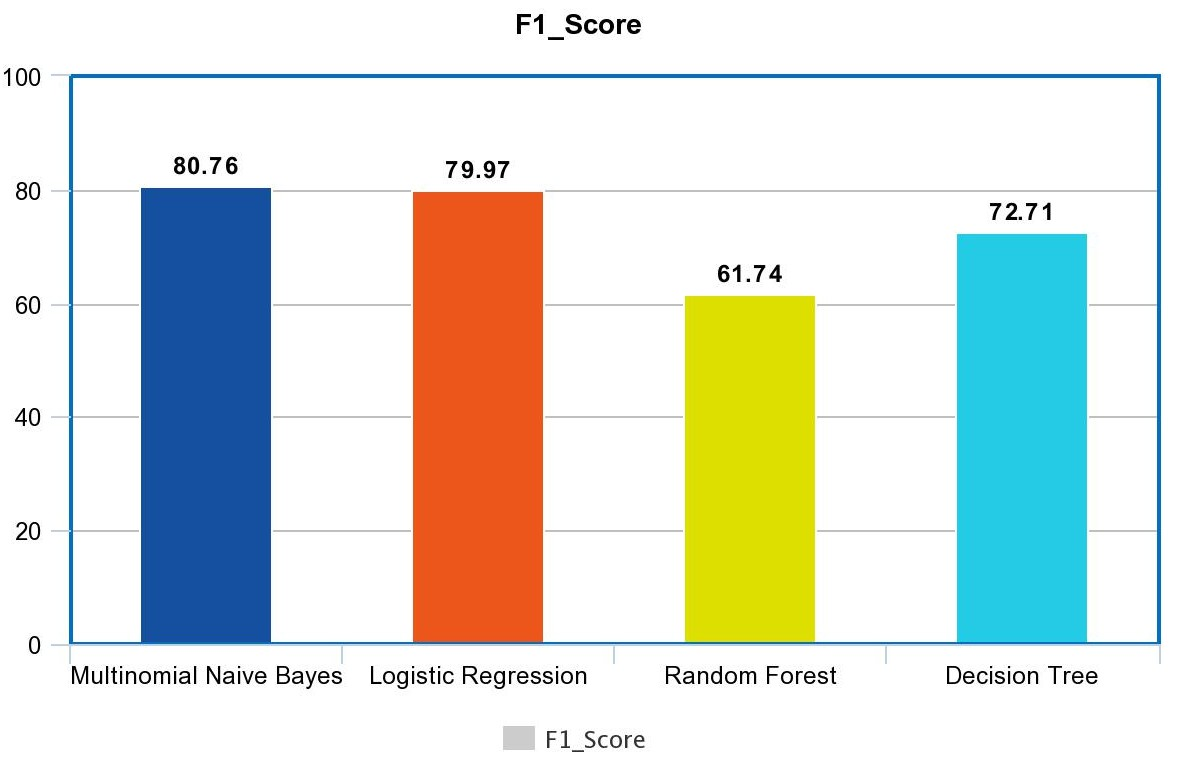
\includegraphics[width= 8cm]{RepeatedKFoldF1_score}
\caption{F1\_Score}
  \label{fig:Repeated KFold F1_score}
\end{figure}

\section{Conclusion}
Distributed Semantic Models provide an approach to find the metaphors in a document(Sentence) based on the context of a phrase that needs to be classified as literal or metaphorical. This paper features an approach to classify a sentence from a set of corpora to be either literal or metaphorical. Features are extracted based on TF-IDF extraction technique. In order to perform the classification, four different classifiers are used namely "Multinomial Naive Bayes", "Decision Tree", "Random Forest" and Logistic Regression(Multinomial) were used. Our experimental results show that out of these classifiers, Multinomial Naive Bayes stands out with accuracy of 84\%. 
\\


\begin{thebibliography}{99}

\bibitem{c1} 
Literal and Metaphorical Senses in Compositional Distributional Semantic Models  \\
\href{http://www.aclweb.org/anthology/P16-1018}
{\textrm{E. Dario Gutierrez, Ekaterina Shutova, Tyler Marghetis, Benjamin K. Bergen, University of California San Diego, University of Cambridge, Indiana University Bloomington]}}

\bibitem{c2} 
From Frequency to Meaning: Vector Space Models of Semantics  \\
\href{https://www.microsoft.com/en-us/research/wp-content/uploads/2017/07/jair10.pdf}
\textrm{Peter D. Turney peter. National Research Council Canada Ottawa, Ontario, Canada, K1A 0R6}

\bibitem{c3}
Feature Extraction TF-IDF
\href{https://medium.freecodecamp.org/how-to-process-textual-data-using-tf-idf-in-python-cd2bbc0a94a3}
\textrm{TF-IDF stands for “Term Frequenct — Inverse Data Frequency”}

\bibitem{c4}
Naive-Bayes-Classifier
\href{http://www.statsoft.com/textbook/naive-bayes-classifier}
{\textrm{The Naive Bayes Classifier technique is based on the so-called Bayesian theorem and is particularly suited when the dimensionality of the inputs is high.}}

\bibitem{c5}
Train Test Split and Cross Validation
\href{https://towardsdatascience.com/train-test-split-and-cross-validation-in-python-80b61beca4b6}
\textrm{In K-Folds Cross Validation we split our data into k different subsets (or folds)}

\bibitem{c6}
Basic-Evaluation-Measures
\href{https://classeval.wordpress.com/introduction/basic-evaluation-measures/}
\textrm{The confusion matrix is a two by two table that contains four outcomes produced by a binary classifier}

\bibitem{c7}
Decision Trees
\href{http://mines.humanoriented.com/classes/2010/fall/csci568/portfolio_exports/lguo/decisionTree.html}
\textrm{The classification technique is a systematic approach to build classification models from an input dat set}

\bibitem{c8}
Saisuresh Krishnakumaran and Xiaojin Zhu. 2007.
{\textrm{Hunting elusive metaphors using lexical resources. In Proceedings of the Workshop on Computational approaches to Figurative Language, pages 13–20. Association for Computational Linguistics.]}}

\bibitem{c9}
Marco Baroni and Roberto Zamparelli. 2010.
\textrm{Nouns are vectors, adjectives are matrices: Representing adjective-noun constructions in semantic space. In Proceedings of the 2010 Conference on Empirical Methods in Natural Language Processing, pages 1183–1193. Association for Computational Linguistics.}

\bibitem{c10}
M. Baroni, S. Bernardini, A. Ferraresi, and E. Zanchetta. 2009.
\textrm{The WaCky wide web: A collection of very large linguistically processed web-crawled corpora. Language Resources and Evaluation}

\bibitem{c11}
Marco Baroni, Raffaela Bernardi, and Roberto Zamparelli. 2014
\textrm{Frege in space: A program of compositional
distributional semantics. Linguistic Issues
in Language Technology.}

\bibitem{c12}
Marco Baroni, Raffaela Bernardi, and Roberto Zamparelli. 2014
\href{https://towardsdatascience.com/decision-trees-and-random-forests-for-classification-and-regression-pt-2-2b1fcd03e342}
\textrm{Random Forests are an ensemble of k untrained Decision Trees (trees with only a root node) with M bootstrap samples.}

\end{thebibliography}

\end{document}
